\documentclass[]{article}
\usepackage{lmodern}
\usepackage{amssymb,amsmath}
\usepackage{ifxetex,ifluatex}
\usepackage{fixltx2e} % provides \textsubscript
\ifnum 0\ifxetex 1\fi\ifluatex 1\fi=0 % if pdftex
  \usepackage[T1]{fontenc}
  \usepackage[utf8]{inputenc}
\else % if luatex or xelatex
  \ifxetex
    \usepackage{mathspec}
  \else
    \usepackage{fontspec}
  \fi
  \defaultfontfeatures{Ligatures=TeX,Scale=MatchLowercase}
\fi
% use upquote if available, for straight quotes in verbatim environments
\IfFileExists{upquote.sty}{\usepackage{upquote}}{}
% use microtype if available
\IfFileExists{microtype.sty}{%
\usepackage{microtype}
\UseMicrotypeSet[protrusion]{basicmath} % disable protrusion for tt fonts
}{}
\usepackage[margin=1in]{geometry}
\usepackage{hyperref}
\hypersetup{unicode=true,
            pdftitle={Análise 1},
            pdfauthor={Raul de Sá Durlo},
            pdfborder={0 0 0},
            breaklinks=true}
\urlstyle{same}  % don't use monospace font for urls
\usepackage{graphicx,grffile}
\makeatletter
\def\maxwidth{\ifdim\Gin@nat@width>\linewidth\linewidth\else\Gin@nat@width\fi}
\def\maxheight{\ifdim\Gin@nat@height>\textheight\textheight\else\Gin@nat@height\fi}
\makeatother
% Scale images if necessary, so that they will not overflow the page
% margins by default, and it is still possible to overwrite the defaults
% using explicit options in \includegraphics[width, height, ...]{}
\setkeys{Gin}{width=\maxwidth,height=\maxheight,keepaspectratio}
\usepackage[normalem]{ulem}
% avoid problems with \sout in headers with hyperref:
\pdfstringdefDisableCommands{\renewcommand{\sout}{}}
\IfFileExists{parskip.sty}{%
\usepackage{parskip}
}{% else
\setlength{\parindent}{0pt}
\setlength{\parskip}{6pt plus 2pt minus 1pt}
}
\setlength{\emergencystretch}{3em}  % prevent overfull lines
\providecommand{\tightlist}{%
  \setlength{\itemsep}{0pt}\setlength{\parskip}{0pt}}
\setcounter{secnumdepth}{5}
% Redefines (sub)paragraphs to behave more like sections
\ifx\paragraph\undefined\else
\let\oldparagraph\paragraph
\renewcommand{\paragraph}[1]{\oldparagraph{#1}\mbox{}}
\fi
\ifx\subparagraph\undefined\else
\let\oldsubparagraph\subparagraph
\renewcommand{\subparagraph}[1]{\oldsubparagraph{#1}\mbox{}}
\fi

%%% Use protect on footnotes to avoid problems with footnotes in titles
\let\rmarkdownfootnote\footnote%
\def\footnote{\protect\rmarkdownfootnote}

%%% Change title format to be more compact
\usepackage{titling}

% Create subtitle command for use in maketitle
\newcommand{\subtitle}[1]{
  \posttitle{
    \begin{center}\large#1\end{center}
    }
}

\setlength{\droptitle}{-2em}
  \title{Análise 1}
  \pretitle{\vspace{\droptitle}\centering\huge}
  \posttitle{\par}
\subtitle{\emph{Homicídios, roubos e furtos de veículos por 100mil habitantes -
Estado de São paulo (2000 - 2010)}}
  \author{Raul de Sá Durlo\footnote{Mestre em Economia - Unesp/FCLAr}}
  \preauthor{\centering\large\emph}
  \postauthor{\par}
  \predate{\centering\large\emph}
  \postdate{\par}
  \date{16 setembro 2017}


\begin{document}
\maketitle
\begin{abstract}
Esta seção tem como objetivo comparar a evolução da criminalidade no
município de São Paulo com as demais regiões do Estado de São Paulo.
Para isso, os municípios do estado de São Paulo são divididos em três
grandes grupos (Interior, Região Metropolitana de São Paulo e Capital).
Os crimes analisados são homocídios, roubo de veículo e furto de
veículo.
\end{abstract}

\section{Introdução}\label{introducao}

Neste \sout{breve} artigo, foi explorada a evolução das taxas de
homicídio, de roubo de veículos e furtos de veículos no Estado de São
Paulo, que por sua vez foi dividido em três grandes grupos: Capital,
Interior, e Grande São Paulo.

O município de São Paulo é destacado em relação aos demais municípios do
estado para justificar sua escolha para análise em relação aos demais.

\section{Metodologia}\label{metodologia}

A metodologia utilizada é a de análise descritiva dos dados. Os dados
referem-se ao número de ocorrências registradas entre os anos de 2000 e
2010 para cada um dos crimes citados. O período analisado vai do ano
2000 até 2010 e a taxa anual foi obtida agregando-se as ocorrências
trimestrais. Como a interpretação de ocorrências criminais é sensível à
mudanças demográficas, os dados foram normalizados em relação à
população residente, sendo calculado, portanto, uma taxa de homicídios
por 100.000 habitantes:

\[txcrime_{tij}=\left(\frac{crime_{tij}}{populacao_{tij}}\right)100000\]

Na equação acima, a taxa de crime no período \(t\) do \(i\)-ésimo crime
é calculada para a localidade \(j\) por 100000 habitantes. Os dados de
ocorrências criminais são provenientes das Estatísticas
Trimestrais\footnote{\url{http://www.ssp.sp.gov.br/estatistica/trimestrais.aspx}}
da Secretaria Estadual de Segurança Pública do Estado de São Paulo. Já
os dados da população residente foram extraídos das Estimativas
utilizadas pelo Tribunal de Contas da União para determinação das cotas
do Fundo de Participação dos Municípios\footnote{\url{http://tabnet.datasus.gov.br/cgi/deftohtm.exe?ibge/cnv/poptsp.def}}.

A criminalidade nas localidades também são analisadas do ponto de vista
das taxas de crescimento composta, que leva em consideração a extensão
do período. Neste caso, a fórmula utilizada foi:

\[txcrescimento=\left(\frac{presente}{passado}\right)^{\left(\frac{1}{n}\right)}-1\]

A escolha de somente três indicadores de ocorrências criminais se deve
principalmete ao fato de haver substantiva subnotificação em relação aos
demais crimes registrados\footnote{Esse é o caso de roubos-outros,
  furtos-outros, tentativas de homicídio e tráfico de entorpecentes. Já
  as ocorrências de latrocínio (roubo seguido de morte) ocorrem em um
  número baixo para o tipo de análise aqui proposta}. Dados de roubo e
furto de veículos também apresentam problemas de interpretação em função
da indisponibilidade de dados de frotas de veículos.

\section{Resultados}\label{resultados}

A tabela abaixo mostra as estatísticas descritivas calculadas para o
período analisado.

\begin{table}[!htbp] \centering 
  \caption{Capital} 
  \label{} 
\begin{tabular}{@{\extracolsep{5pt}}lccccc} 
\\[-1.8ex]\hline 
\hline \\[-1.8ex] 
Statistic & \multicolumn{1}{c}{N} & \multicolumn{1}{c}{Mean} & \multicolumn{1}{c}{St. Dev.} & \multicolumn{1}{c}{Min} & \multicolumn{1}{c}{Max} \\ 
\hline \\[-1.8ex] 
tx\_homicidio & 11 & 27.76 & 16.32 & 10.64 & 53.22 \\ 
tx\_furto & 11 & 474.90 & 74.07 & 381.94 & 605.90 \\ 
tx\_roubo & 11 & 392.81 & 95.54 & 286.95 & 614.81 \\ 
\hline \\[-1.8ex] 
\end{tabular} 
\end{table}

\begin{table}[!htbp] \centering 
  \caption{Grande SP} 
  \label{} 
\begin{tabular}{@{\extracolsep{5pt}}lccccc} 
\\[-1.8ex]\hline 
\hline \\[-1.8ex] 
Statistic & \multicolumn{1}{c}{N} & \multicolumn{1}{c}{Mean} & \multicolumn{1}{c}{St. Dev.} & \multicolumn{1}{c}{Min} & \multicolumn{1}{c}{Max} \\ 
\hline \\[-1.8ex] 
tx\_homicidio & 11 & 27.13 & 13.24 & 12.22 & 46.17 \\ 
tx\_furto & 11 & 245.46 & 32.57 & 203.40 & 299.95 \\ 
tx\_roubo & 11 & 270.61 & 85.21 & 188.28 & 448.08 \\ 
\hline \\[-1.8ex] 
\end{tabular} 
\end{table}

\begin{table}[!htbp] \centering 
  \caption{Interior} 
  \label{} 
\begin{tabular}{@{\extracolsep{5pt}}lccccc} 
\\[-1.8ex]\hline 
\hline \\[-1.8ex] 
Statistic & \multicolumn{1}{c}{N} & \multicolumn{1}{c}{Mean} & \multicolumn{1}{c}{St. Dev.} & \multicolumn{1}{c}{Min} & \multicolumn{1}{c}{Max} \\ 
\hline \\[-1.8ex] 
tx\_homicidio & 11 & 14.10 & 4.73 & 8.51 & 20.35 \\ 
tx\_furto & 11 & 179.66 & 8.11 & 165.80 & 198.17 \\ 
tx\_roubo & 11 & 78.55 & 16.72 & 61.31 & 120.88 \\ 
\hline \\[-1.8ex] 
\end{tabular} 
\end{table}

Abaixo o gráfico com a evolução tas taxas de crime. É notória a queda
nos himicídios, da magnitude de -7.117956\% no interior do estado,
-12.4470107\% na região metropolitana e -14.8721999\% na capital
paulista.

\newpage

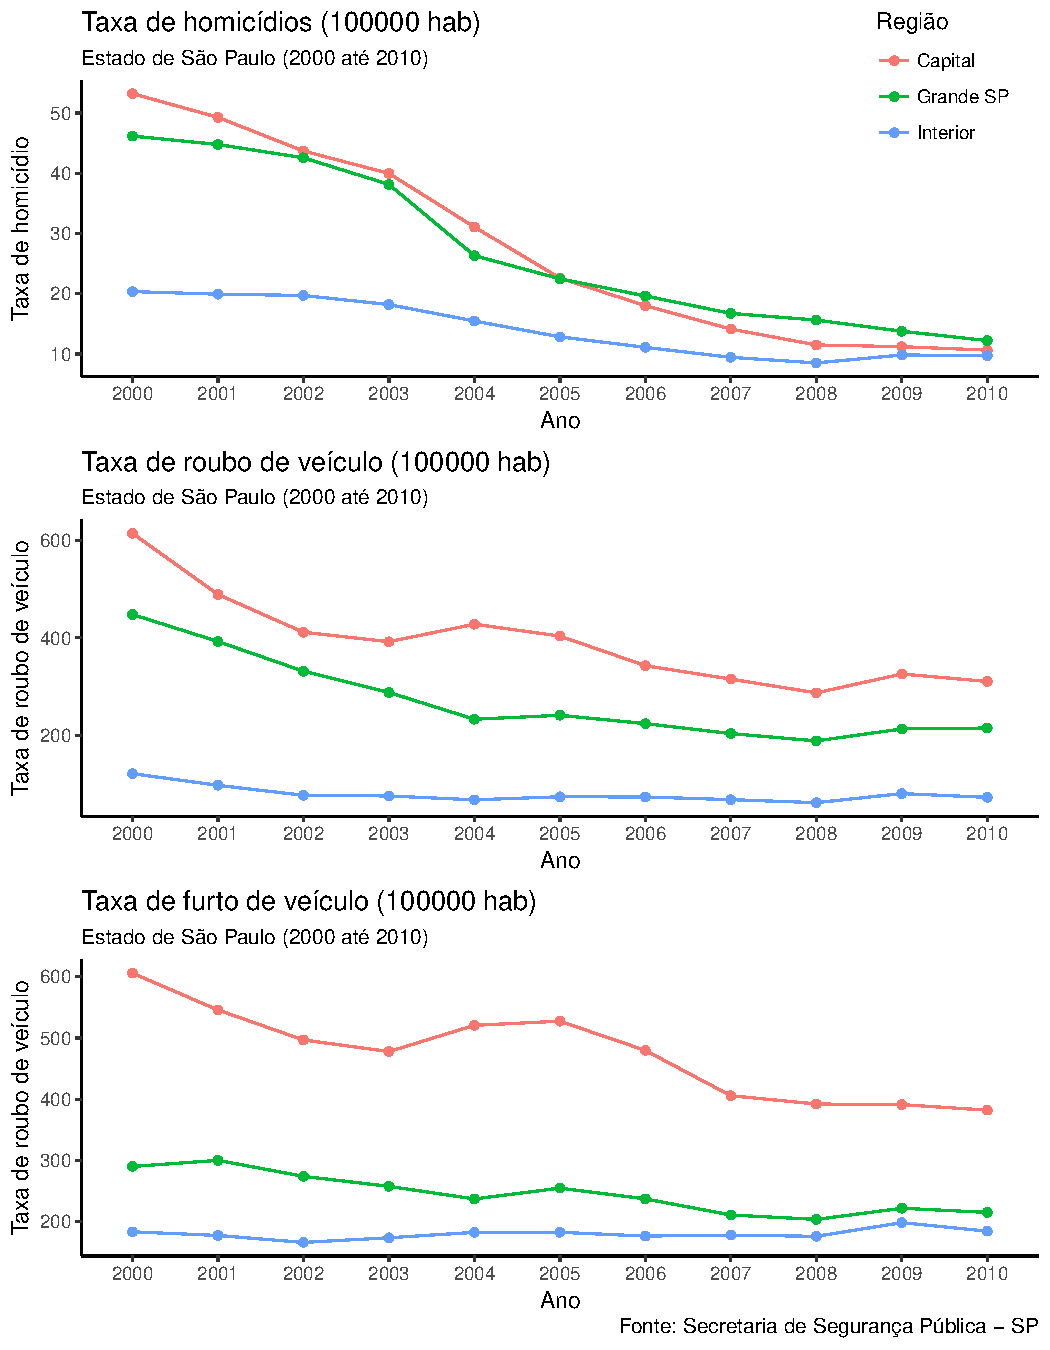
\includegraphics{Análise_1_files/figure-latex/Gráficos-1.pdf}

\newpage

\section{Discussão}\label{discussao}

A diferença entre as taxas de crimes entre as cidades do interior do
estado e a capital São Paulo se contrasta com as discussões que tratam
sobre a influência das características locais (ou intra-urbanas) sobre o
crime em uma determinada localidade. Glaeser and Sacerdote (1999), por
exemplo, chama a atenção para a correlação entre o tamanho das cidades e
as altas taxas de criminalidade e, aparentemente, isso pode estar
relacionado à questões de ambiente e interações sociais que ocorrem nos
ambientes urbano. Oliveira (2005) faz argumentação semelhante para o
caso das cidades brasileiras no ano de 2010. Eck and Weisburd (2015)
argumenta que, cada vez mais, a composição do ambiente ou as
características locais \emph{(crime places)} tem chamado a atenção de
criminologistas e estudiosos do tema.

Apesar de haverem estudos sobre as taxas de crimes no município de São
Paulo, pouco se tem discutido sobre a influencia das características
urbanas na determinação do padrão de criminalidade na cidade.

\section{Conclusão}\label{conclusao}

\section*{Referências Bibliográficas}\label{referencias-bibliograficas}
\addcontentsline{toc}{section}{Referências Bibliográficas}

\hypertarget{refs}{}
\hypertarget{ref-eck2015crime}{}
Eck, John E, and David L Weisburd. 2015. ``Crime Places in Crime
Theory.''

\hypertarget{ref-glaeser1999there}{}
Glaeser, Edward L, and Bruce Sacerdote. 1999. ``Why Is There More Crime
in Cities?'' \emph{Journal of Political Economy} 107 (S6). The
University of Chicago Press: S225--S258.

\hypertarget{ref-de2005criminalidade}{}
Oliveira, Cristiano Aguiar de. 2005. ``Criminalidade E O Tamanho Das
Cidades Brasileiras: Um Enfoque Da Economia Do Crime.'' In \emph{Anais
Do Xxxiii Encontro Nacional de Economia {[}Proceedings of the 33th
Brazilian Economics Meeting{]}}. 152. ANPEC-Associação Nacional dos
Centros de Pósgraduação em Economia {[}Brazilian Association of Graduate
Programs in Economics{]}.


\end{document}
